% !TEX root = ../thesis-example.tex
%
\chapter{Représentation visuelle}
\label{ch:visual_representation}

\cleanchapterquote{Ces petits morceaux d’espace visuels,\\
dont la connexion n’est pas donnée d’avance, \\
par quoi voulez vous qu’ils soient connectés, \\
sinon par la main?}{Gilles Deleuze}{\textit{Qu'est ce que l'acte de création?}\\ conférence donnée à la FEMIS \cite{deleuze_deux_2003}}

voir mp.TUI.key pour les images à inclure

%%%%%%%%%%%%%%%%%%%%%%%%%%%%%%%%%%%%%%%%%
\section{le cockpit du musicien?}
Si un DMI présente une une certaine ergonomie physique, avec un agencement stable de certains éléments d'interaction, les écrans permettent l'affichage d'un certain nombre d'éléments dynamiques qui peuvent également être support d'interaction, que cela soit avec le clavier, la souris, une interface de contrôle MIDI ou encore l'écran lui-même quand il est tactile.

Ces éléments virtuels permettent :
\vspace{-1em}
\begin{itemize}[noitemsep]
	\item d'étendre considérablement le champ des opérations possibles, en proposant un espace virtuel beaucoup plus grand, grâce à des systèmes d'onglets, de fenêtres multiples, de menus condensant différentes options;
	\item d'afficher des éléments dynamiques tels que l'état d'avancement d'un séquenceur;
	\item d'adapter l'ergonomie de l'interface à un contexte particulier, e.g. en duplicant des éléments de GUI pour permettre un jeu à plusieurs sur une même interface;
\end{itemize}

%%%%%%%%%%%%%%%%%%%%%%%%%%%%%%%%%%
\section{Aspects visuels du design d'instrument}

La conception d'un instrument englobe plusieurs aspects qui affectent son aspect visuel. Je passerai en revue quelques-uns de ces aspects, en prenant des exemples des instruments acoustiques, comme rétrospective sur ce qui nous a conduit aux développements que nous sommes en train de faire avec les \glspl{DMI}.

\subsection{liés à la production du son}

La conception des instruments se préoccupe de la qualité du son. Bien que cela soit particulièrement évident pour les instruments acoustiques dont la forme a des conséquences directes sur le rendement sonore (comme le montre la figure \ref{fig:visual_representation:fhole}), les formes particulières issues de la lutherie traditionnelle ont également donné naissance à un certain nombre d'éléments iconiques (par exemple, les ouïes du violons) et de facteurs de forme (par exemple, une taille plus grande donne un ton grave) associés à l'idée d'un instrument. De plus, les DMI peuvent intégrer des transducteurs acoustiques, tels que des microphones piézoélectriques ou des haut-parleurs tactiles, qui influencent la conception acoustique de leurs composants matériels.

%------------ Figure : f-hole et boehm -----------
\begin{figure}[!htbp]
	\captionsetup{format=plain}%
	\centering
	\begin{minipage}[t]{0.48\textwidth}
		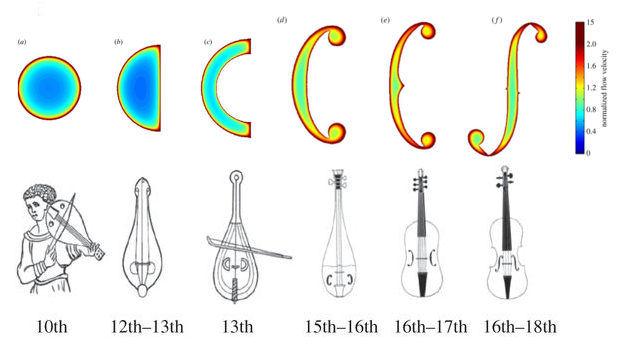
\includegraphics[width=\linewidth]{gfx/06_visual_representation/f-hole.png}
		\caption{évolution de la forme des ouïes du violon d'après \cite{nia_evolution_2015}}
		\label{fig:visual_representation:fhole}
	\end{minipage}
	\hspace{.02\linewidth}
	\begin{minipage}[t]{0.48\textwidth}
	    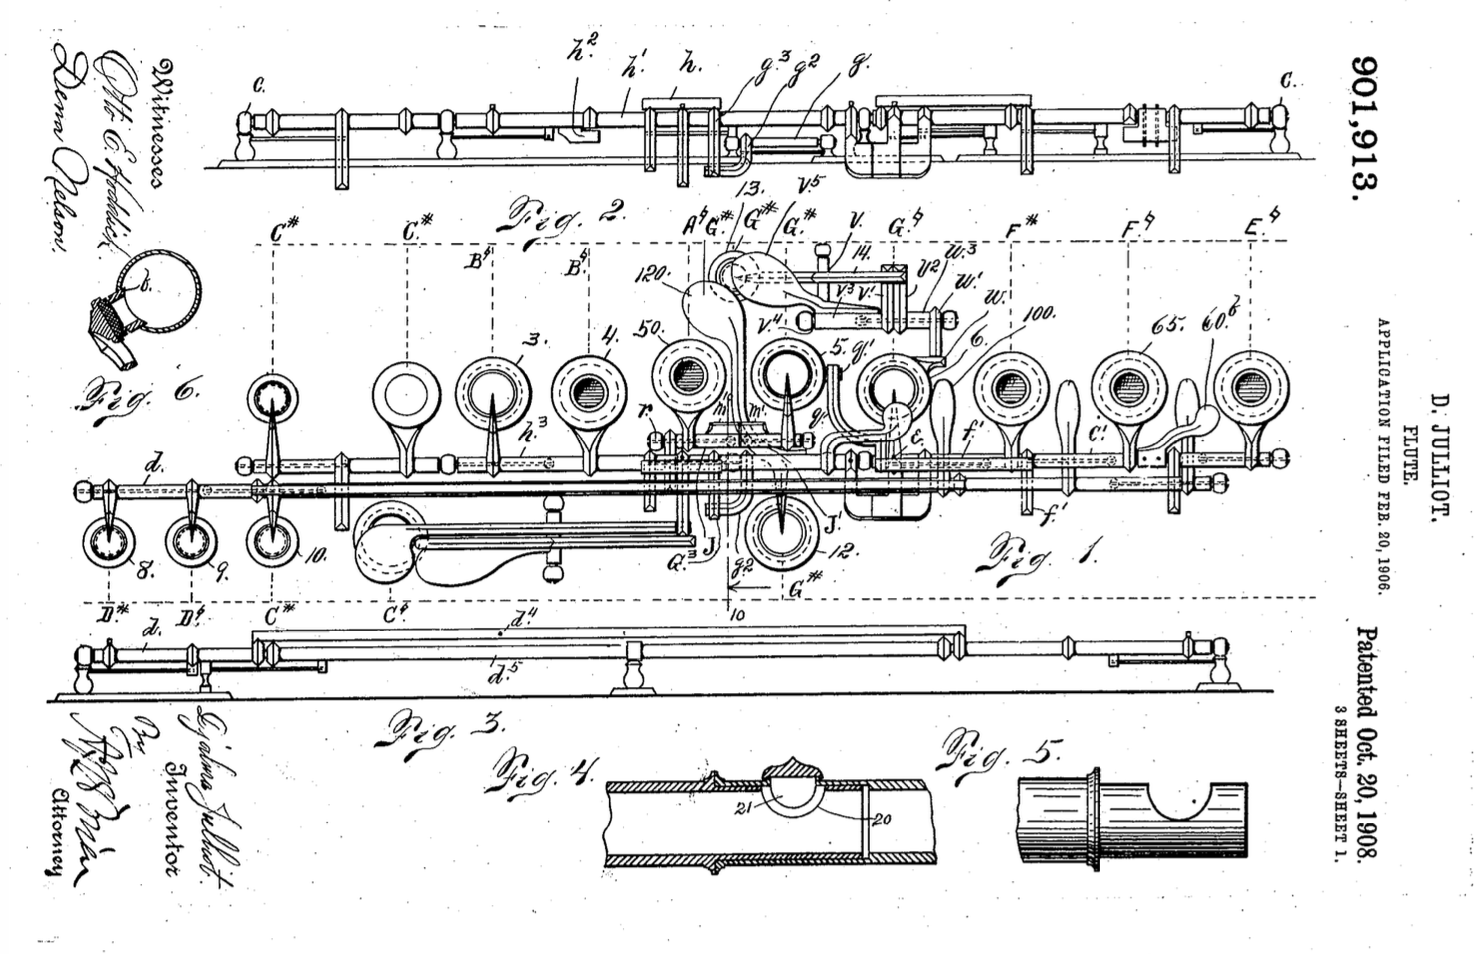
\includegraphics[width=\linewidth]{gfx/06_visual_representation/Julliot_patent.png}
		\caption{Extrait du brevet de J. Djalma sur \iquote{l'amélioration du clétage des flûtes de Boehm}, 1908.}
		\label{fig:visual_representation:boehm}
	\end{minipage}
\end{figure}

\subsection{Adaptations ergonomiques}

L'instrument s'adapte également au corps. Un exemple intéressant est l'évolution du traverso vers la flûte de concert occidentale, à l'aide du système Boehm dans les années 1840 (cf. figure \ref{fig:visual_representation:boehm}). Ce système de clavetage découple la topologie gestuelle de la topologie du flux d'air et de la topologie de résonance. En utilisant des manches et des platines, il permettait d'améliorer le son en faisant des trous plus grands et en les plaçant à des endroits adéquats pour la résonance, tandis que les touches pouvaient être placées à des endroits pratiques pour les mains de la flûtiste.
Le système Boehm peut être qualifié de "modèle intermédiaire" entre le geste et la production sonore, fait d'un système mécanique dans ce cas. La plupart des instruments combinent divers "modèles intermédiaires" pour amplifier, enrichir, déplacer, focaliser, multiplier les gestes des interprètes et générer des mouvements hors du champ des possibilités du corps humain : pédales de grosse caisse, marteaux et amortisseurs pour piano, archets et plectras, etc.

\subsection{Intégration de la théorie musicale}

%------------ Figure : keyboard et TUI - scale -----------
\begin{figure}[!htbp]
	\captionsetup{format=plain}%
	\centering
	\begin{minipage}[t]{0.48\textwidth}
		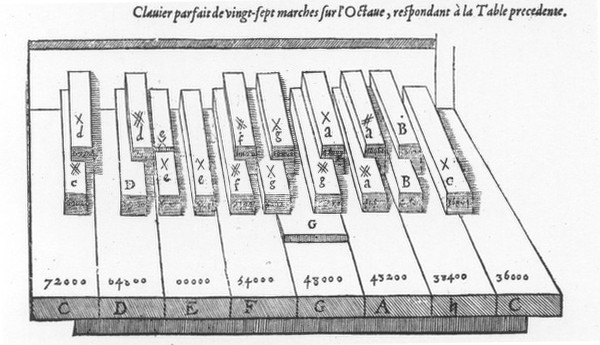
\includegraphics[width=\linewidth]{gfx/06_visual_representation/Mersenne_clavier.png}
		\caption{Twenty-seven-steps keyboard invented by Mersenne (1636)}
		\label{fig:visual_representation:MersenneKeyboard}
	\end{minipage}
	\hspace{.02\linewidth}
	\begin{minipage}[t]{0.48\textwidth}
	    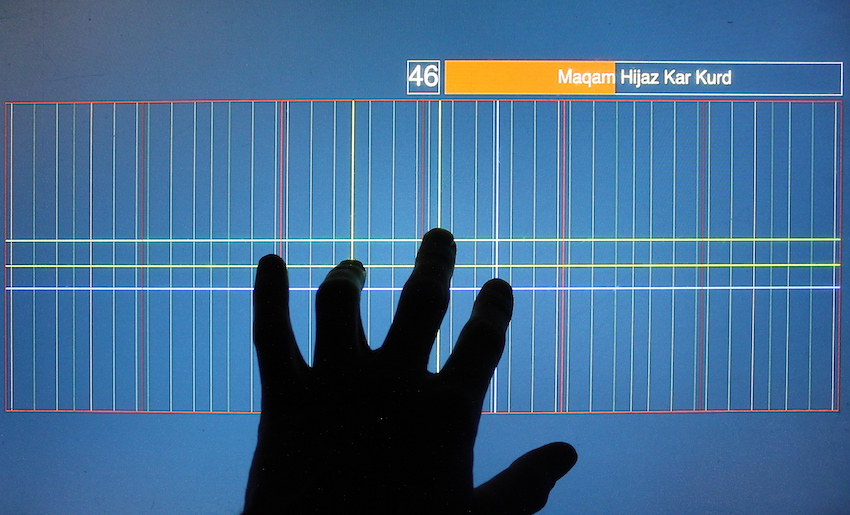
\includegraphics[width=\linewidth]{gfx/06_visual_representation/mpTUI_pitchgrid_72dpi.png}
		\caption{Une grille de hauteur avec une représentation micro-tonale réalisée avec mp.TUI. La luminosité des lignes verticales varie en fonction de la quantité de quantification.}
		\label{fig:visual_representation:pitch_grid}
	\end{minipage}
\end{figure}

Les instruments de musique intègrent également des éléments de théorie musicale. Par exemple, la partie supérieure d'un clavier (touches noir et blanc) représente la gamme chromatique, tandis que la partie inférieure (touches blanches seulement) représente la gamme diatonique en do majeur. Le dimensionnement et le positionnement de ces touches est un compromis intéressant entre les contraintes mécaniques du système de marteaux et une représentation uniforme des échelles diatonique et chromatique. De plus, la largeur de l'octave est telle qu'elle tient sous une main tendue, ce qui permet de jouer n'importe quel intervalle à l'intérieur d'une octave avec une seule main, reflétant en quelque sorte l'équivalence des octaves. Les claviers ont fait l'objet de nombreuses expérimentations avec des systèmes de hauteur micro-tonale, des intonations et des mises en page de notes, utilisant des grilles hexagonales ou plusieurs couches de touches (figure \ref{fig:visual_representation:MersenneKeyboard}). En tant que système symbolique, une telle théorie musicale peut être facilement encodée dans les ordinateurs. Les logiciels de production musicale contiennent tellement de fonctions et de règles basées sur la théorie musicale qu'elles s'adaptent difficilement à l'interface. Thor Magnusson parle d'" outils épistémiques " pour décrire le DMI, affirmant qu'il est conçu avec " un tel degré de pertinence symbolique qu'il devient un système de connaissance et de pensée dans ses propres termes " (Magnusson, 2009). En tant que tel, ce "système de connaissances" est un paysage imaginaire à explorer, un territoire sonore pour lequel l'interface et la cartographie de l'instrument peuvent métaphoriquement se présenter comme une carte.

\subsection{Adaptations au contexte de performance}
Si l'on élargit un peu la notion d'instrument de musique pour les considérer simplement comme des outils pour faire de la musique, alors les partitions, les salles de concert, le public et plus généralement, le contexte de la performance participent aussi et influencent la conception des instruments. Les partitions orientées (figure \ref{fig:visual_representation:table_music}) sont un exemple d'adaptation de la partition au contexte de la "musique de table", permettant dans ce cas aux musiciens de lire la partition lorsqu'ils sont assis autour d'une table. De même, les DMI sur écran peuvent adapter leur disposition au nombre d'interprètes en présentant à chacun d'eux un groupe d'éléments d'interface utilisateur orientés vers eux (figure \ref{fig:visual_representation:multi_orientation}).

%------------ Figure : keyboard et TUI - scale -----------
\begin{figure}[!htbp]
	\captionsetup{format=plain}%
	\centering
	\begin{minipage}[t]{0.48\textwidth}
		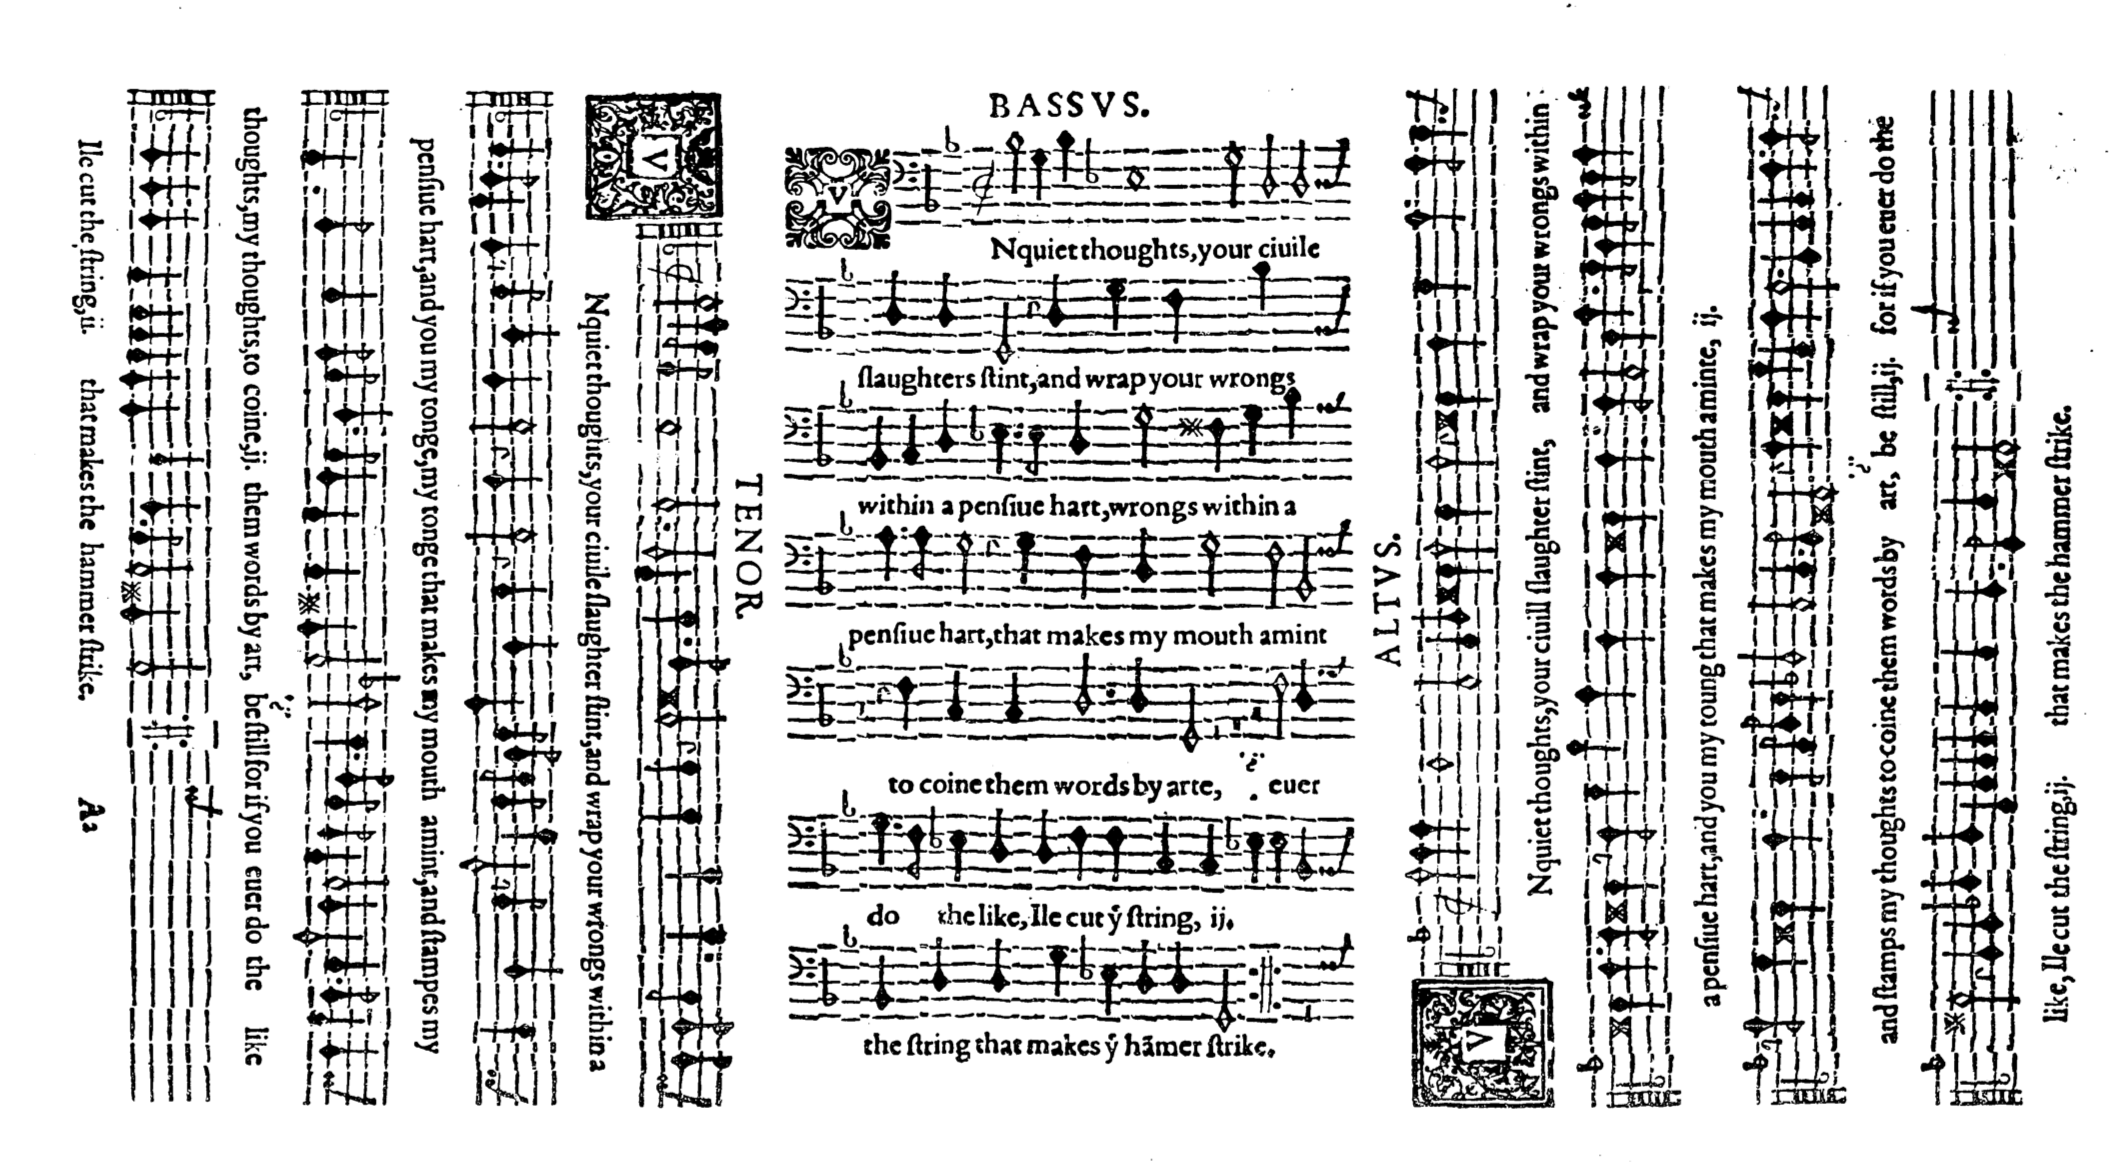
\includegraphics[width=\linewidth]{gfx/06_visual_representation/Dowland-firstBookOfSonges.png}
		\caption{Twenty-seven-steps keyboard invented by Mersenne (1636)}
		\label{fig:visual_representation:table_music}
	\end{minipage}
	\hspace{.02\linewidth}
	\begin{minipage}[t]{0.48\textwidth}
	    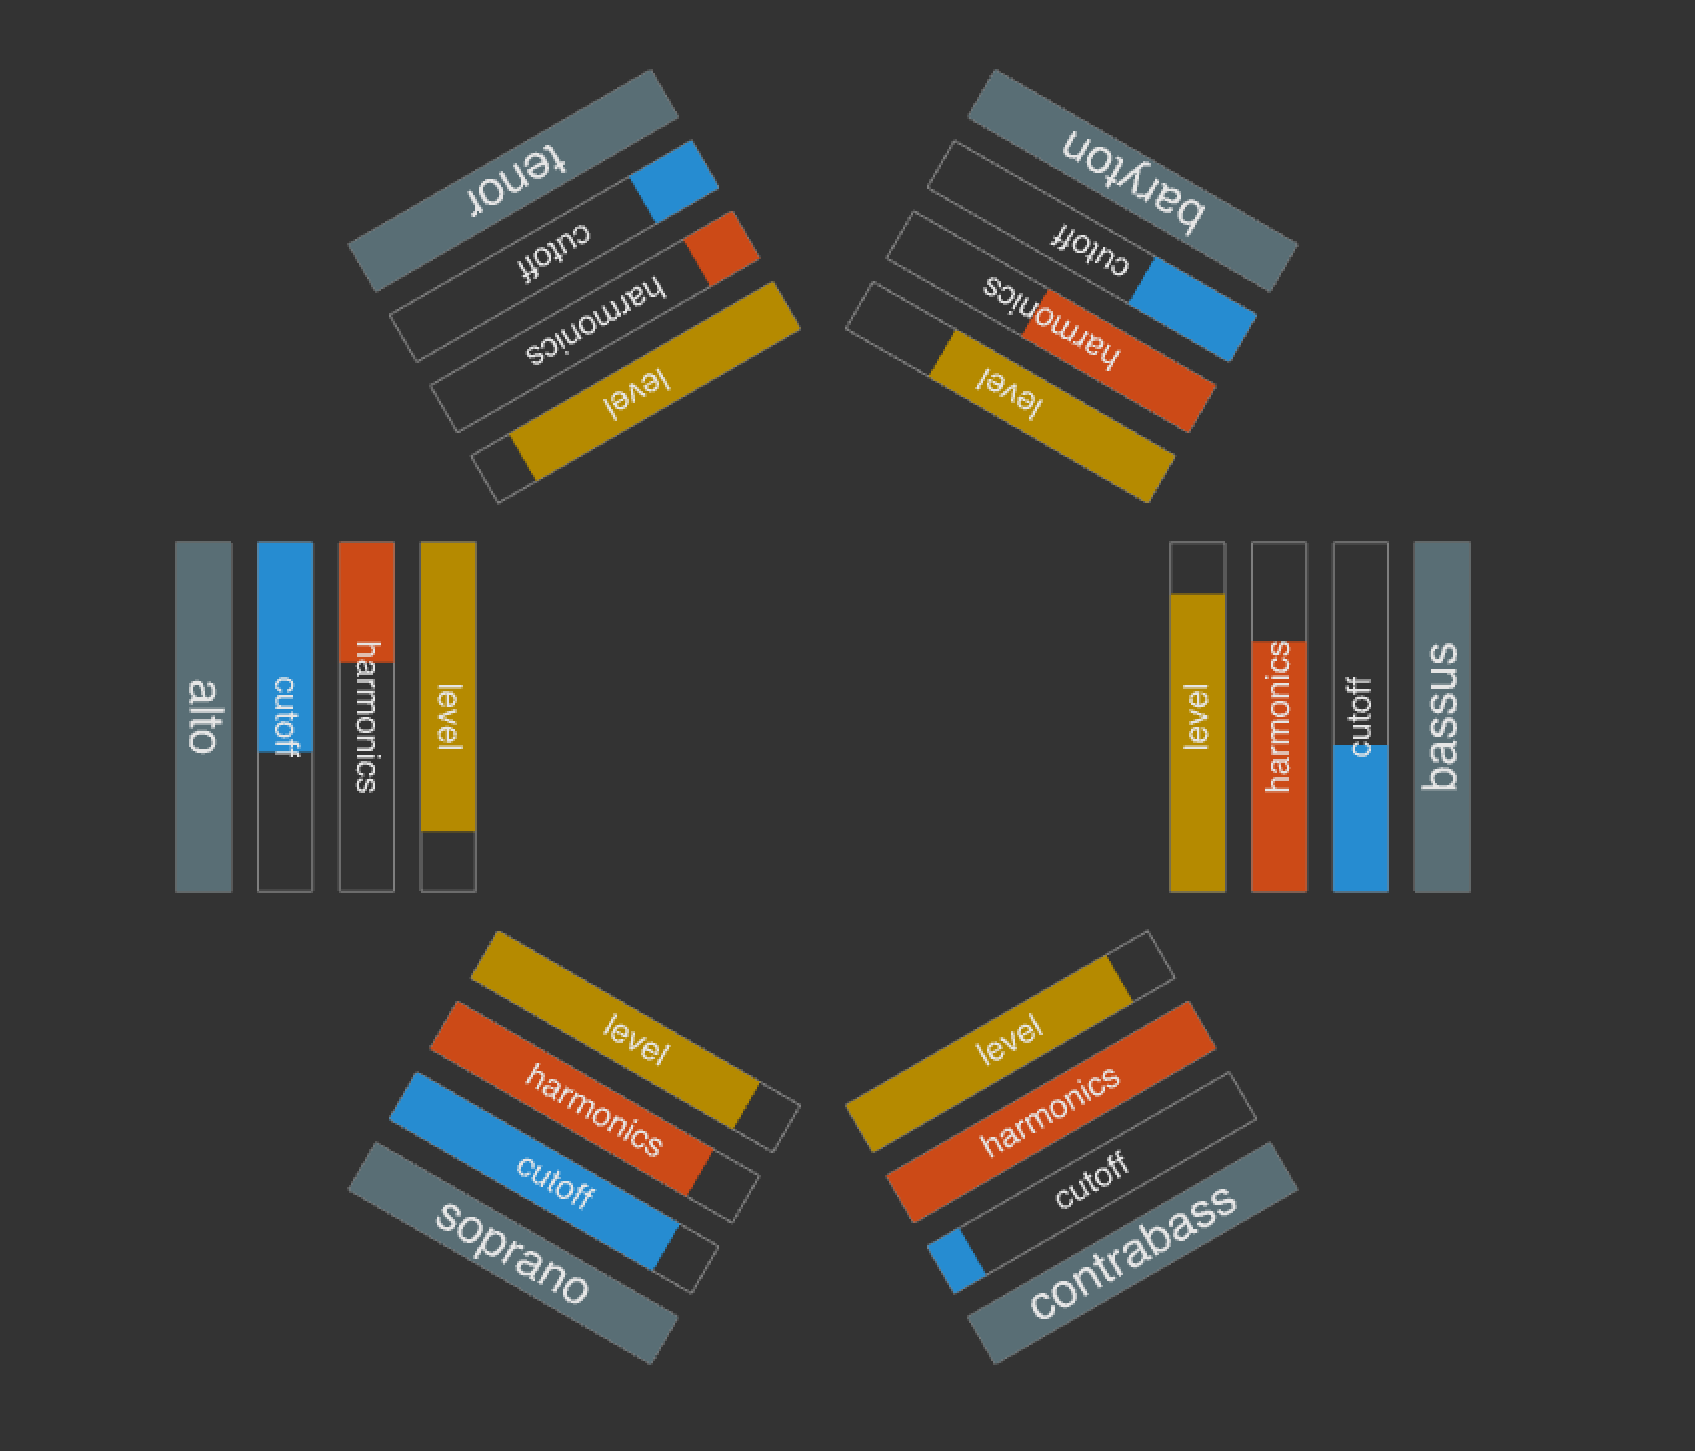
\includegraphics[width=\linewidth]{gfx/06_visual_representation/mpTUI_multi-orientation.png}
		\caption{Instrument simple adaptée pour 6 joueurs située autour d'une interface commune.}
		\label{fig:visual_representation:multi_orientation}
	\end{minipage}
\end{figure}

\subsection{Adaptations à l'expérimentation}
En fin de compte, le processus de conception des instruments de musique contient une grande part de travail empirique. Le processus d'ajustement des réglages d'un instrument nécessitera souvent une rétroaction directe pour les réglages fins faits à la main, jusqu'à ce qu'il sonne et se prête au jeu.


%%%%%%%%%%%%%%%%%%%%%%%%%%%%%%%%%%%%%%%%%
\section{le cockpit du musicien?}
\label{sec:visual_representation:sec1}
\cite{vertegaal_towards_1996}
Interfaces héritées de l'ingénierie sonore avec leur quantité de commandes indépendantes et ordonnées.

%%%%%%%%%%%%%%%%%%%%%%%%%%%%%%%%%%%%%%%%%
\section{Guides, carte, fretting}

Apprendre indépendamment de la transposition
\iquote{I love the piano sound but not the difficulty of learning the variations from one key to another.  The LinnStrument with its 4th tuning avoids all of those issues.} Jeff Moen about the linnstrument (\url{http://jeffmoen.com/how_i_got_here.html})

Passage du "savoir le contenu" à "savoir que ce contenu existe" et "savoir le chercher".
Savoir cartographique.

%%%%%%%%%%%%%%%%%%%%%%%%%%%%%%%%%%%%%%%%%
\section{représentation de l'objet/processus virtuel}
La musique recourt parfois à l'utilisation de processus pour le développement musical. 
\subsection{visualisation pour le public}
cf. De Laubier: Bach déploiement de la forme et cadence rendues visibles.

\subsection{interaction avec la visualisation}
cf. Goudard: FIB\_R

%%%%%%%%%%%%%%%%%%%%%%%%%%%%%%%%%%%%%%%%%
\section{intégration de la partition dans l'interface}
Screen scores, patterns de séquenceur, cues de déclenchement, presets

%%%%%%%%%%%%%%%%%%%%%%%%%%%%%%%%%%%%%%%%%
\section{aspects esthétiques / instruments visuels}
En tant qu'élément scénographique, la représentation visuelle joue un rôle dans l'esthétique et la poésie de l'instrument. Le design de l'interface visuelle de l'instrument ne se résume ainsi pas à un design fonctionnel\\

Exemple dans FIB\_R : toute la performance visuelle re-projetée sur l'écran correspond à ce que les instrumentistes ont face à eux sur leur tablette. A la fois espace d'interaction et création visuelle esthétique/poétique.



%%%%%%%%%%%%%%%%%%%%%%%%%%%%%%%%%%%%%%%%%
\section{La librairie mp.TUI pour Max}

\subsection{Motivations}

ré-inventer la route (ou le slider) : les interactions prévues dans les éléments de GUI de la bureautique ne sont pas conçues pour l'interaction musicale. Adaptation ad-hoc du comportement de GUI. Exemple d'un slider avec mémoire du dernier doigt. 

\todo{inclure les figures de la présentation mp.TUI.key}

\subsection{Utilisation de MP pour le contrôle multitouch de GUI}

La bibliothèque mp.TUI\footnote{Sources disponible sur \url{https://github.com/LAM-IJLRA/ModularPolyphony-TUI/}.} est construite sur le protocole MP (cf. \ref{sec:algorithms:MP}). Elle fournit un cadre basé sur les logiques de patch de Max pour créer de nouveaux composants d'interface utilisateur multitouch dans un contexte OpenGL et surmonter certaines limitations de l'interface graphique native de l'environnement de patching de Max. Par exemple, les interfaces graphiques sont généralement orientées sur une disposition horizontale/verticale avec une orientation de lecture du haut vers le bas alors qu'on peut souhaiter avoir plusieurs orientations, comme dans la situation présentée sur la figure \ref{fig:visual_representation:multi_orientation}. La superposition de divers composants peut nécessiter des couleurs et des transparents personnalisés, et l'on peut souhaiter inclure des interfaces visuelles plus complexes que les curseurs et les boutons, par exemple des particules, des vidéos, des modèles 3d, des shaders (cf. figure \ref{fig:visual_representation:phonetogramme}), etc.

Les composants de la bibliothèque sont d'un ensemble d'abstractions de trois types :
\vspace{-1em}
\begin{itemize}[noitemsep]
	\item \textbf{des composants système}, qui implémentent les fonctions essentielles pour envelopper les graphiques dans un élément cliquable. Cela inclut le "mp.TUI.hub" qui récupère les données de l'interaction de la souris sur la fenêtre OpenGL ainsi que les messages TUIO reçus par UDP et les envoie aux composants graphiques sélectionnés.;
	\item \textbf{des éléments de GUI}, qui sont des instances prêtes à l'emploi de widgets courants ou moins courants tels que curseurs, claviers, graphes, etc.;
	\item \textbf{des outils}, un ensemble d'abstractions qui permettent de créer facilement de nouveaux composants en proposant des fonctions utiles pour la conception d'interaction (transformation de la visualisation, gestion de la polyphonie sur un élément, interaction tels que pinch-zoom, calcul de dérivées, etc.).
\end{itemize}

\subsection{Les composants de la librairie mp.TUI}

Les composants utilisent des transformations géométriques hiérarchiques\footnote{à l'aide de l'objet jit.anim.node de Max}, qui permet d'obtenir des coordonnées relatives au monde ou à l'objet indépendamment de la position, de l'échelle et de l'orientation du composant de l'interface utilisateur. Cela permet également de créer des groupes de composants, comme on le ferait dans n'importe quel logiciel de CAO. Suivant la nature empirique de la lutherie numérique revendiquée ci-dessus, un "mode édition" est également disponible pour manipuler rapidement à la main la position, l'échelle et l'orientation des composants de l'interface utilisateur (figure \ref{fig:visual_representation:groups_patch} et \ref{fig:visual_representation:groups}).

%-------------------------- Figure : phonetogramme ----------------------------------
\begin{figure}[!htbp]
	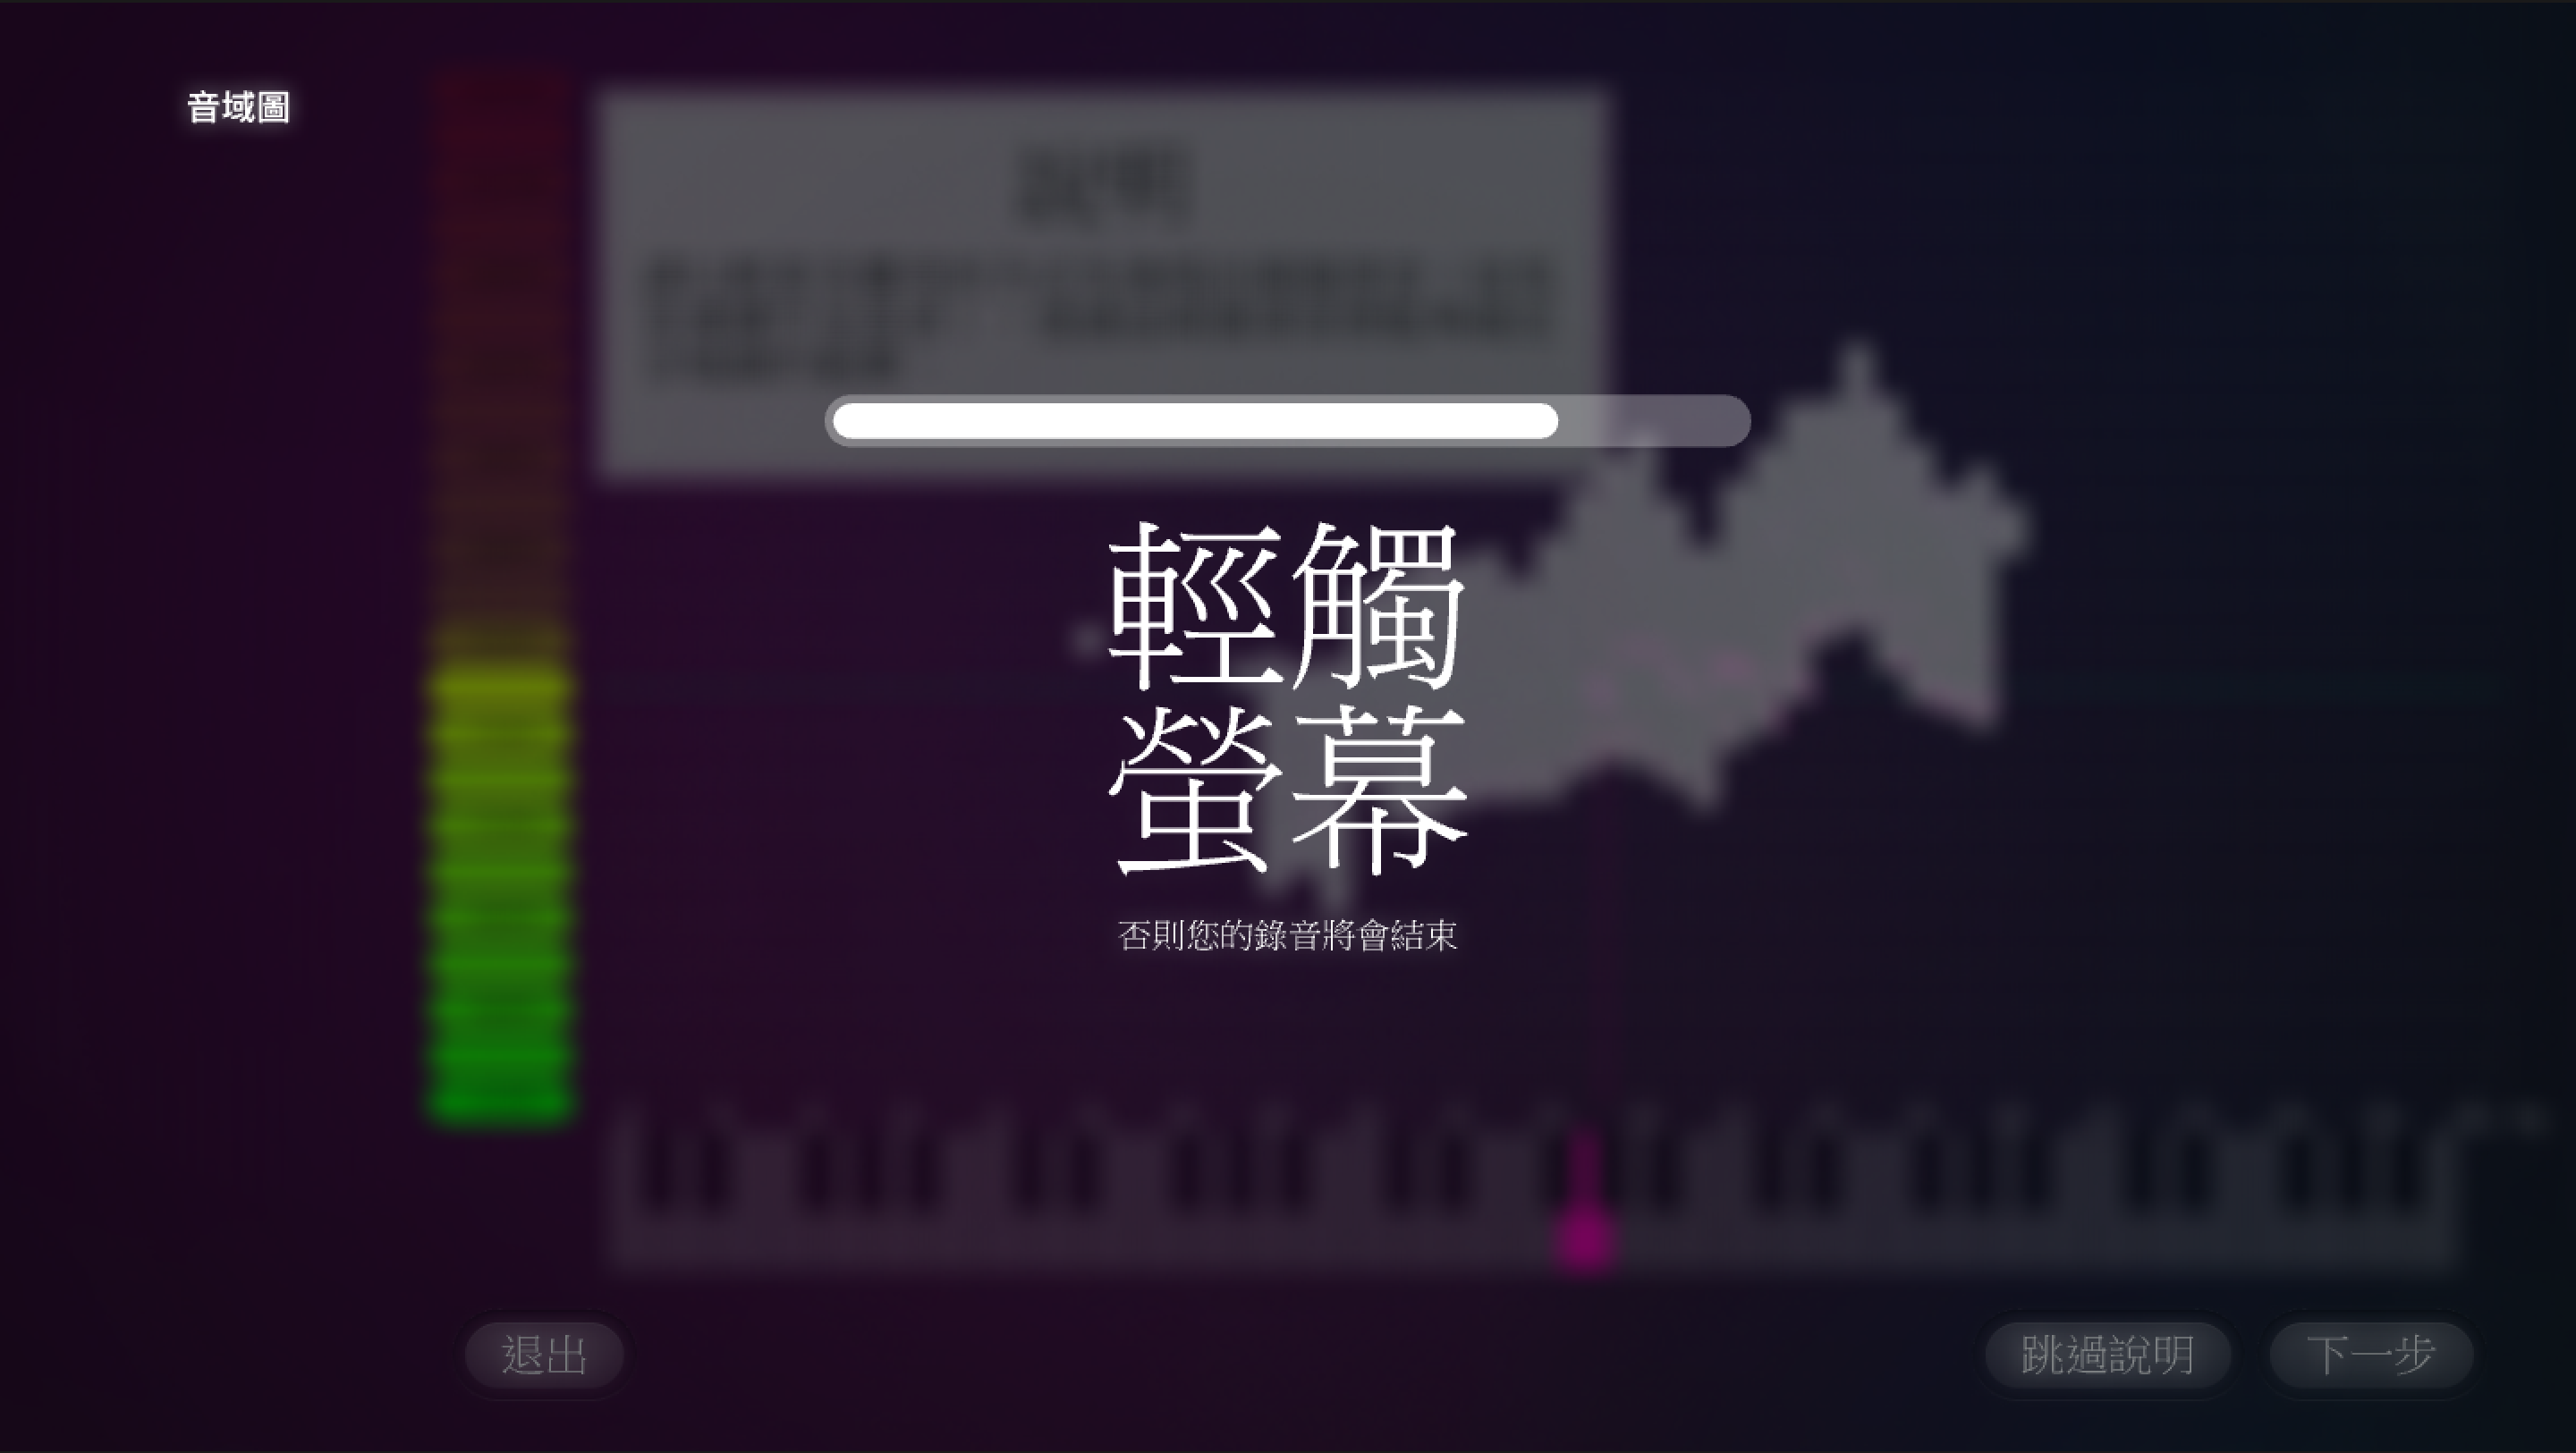
\includegraphics[width=\textwidth]{gfx/06_visual_representation/Phonetogramme.png}
	\caption{``Le phonetogramme'', une application muséographique conçue pour la Cité des Sciences, dont la GUI est réalisée avec la librairie mp.TUI.}
	\label{fig:visual_representation:phonetogramme}
\end{figure}

La possibilité de concevoir des objets audiovisuels en Max en étroite relation avec la programmation de l'interaction entre le geste, l'audio et le visuel permet de les intégrer dans des scénarios dynamiques personnalisés : histoires narratives pour des ateliers éducatifs avec des enfants, scénarios réactifs, visualisations personnalisées pour les malvoyants, expositions muséographiques avec chartes graphiques spécifiques, adaptation réactive aux formats d'écran, graphismes expérimentaux pour l'esthétique des performances artistiques live, etc.


%------------------ Figure : mp.TUI : simple slider ---------------------
\begin{figure}[!htbp]
	\makebox[\linewidth][c]{%
		\begin{subfigure}[b]{.5\textwidth}
			\centering
			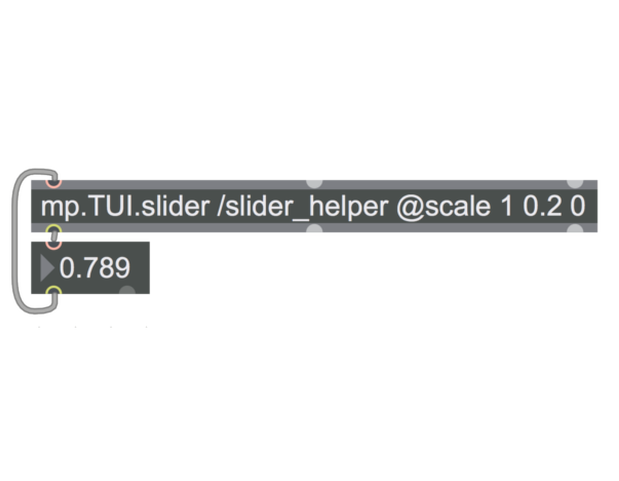
\includegraphics[width=.95\textwidth]{gfx/06_visual_representation/mpTUI_slider-patcher.png}
			\caption{L'objet Max créant un slider}
		\end{subfigure}%
		\begin{subfigure}[b]{.5\textwidth}
			\centering
			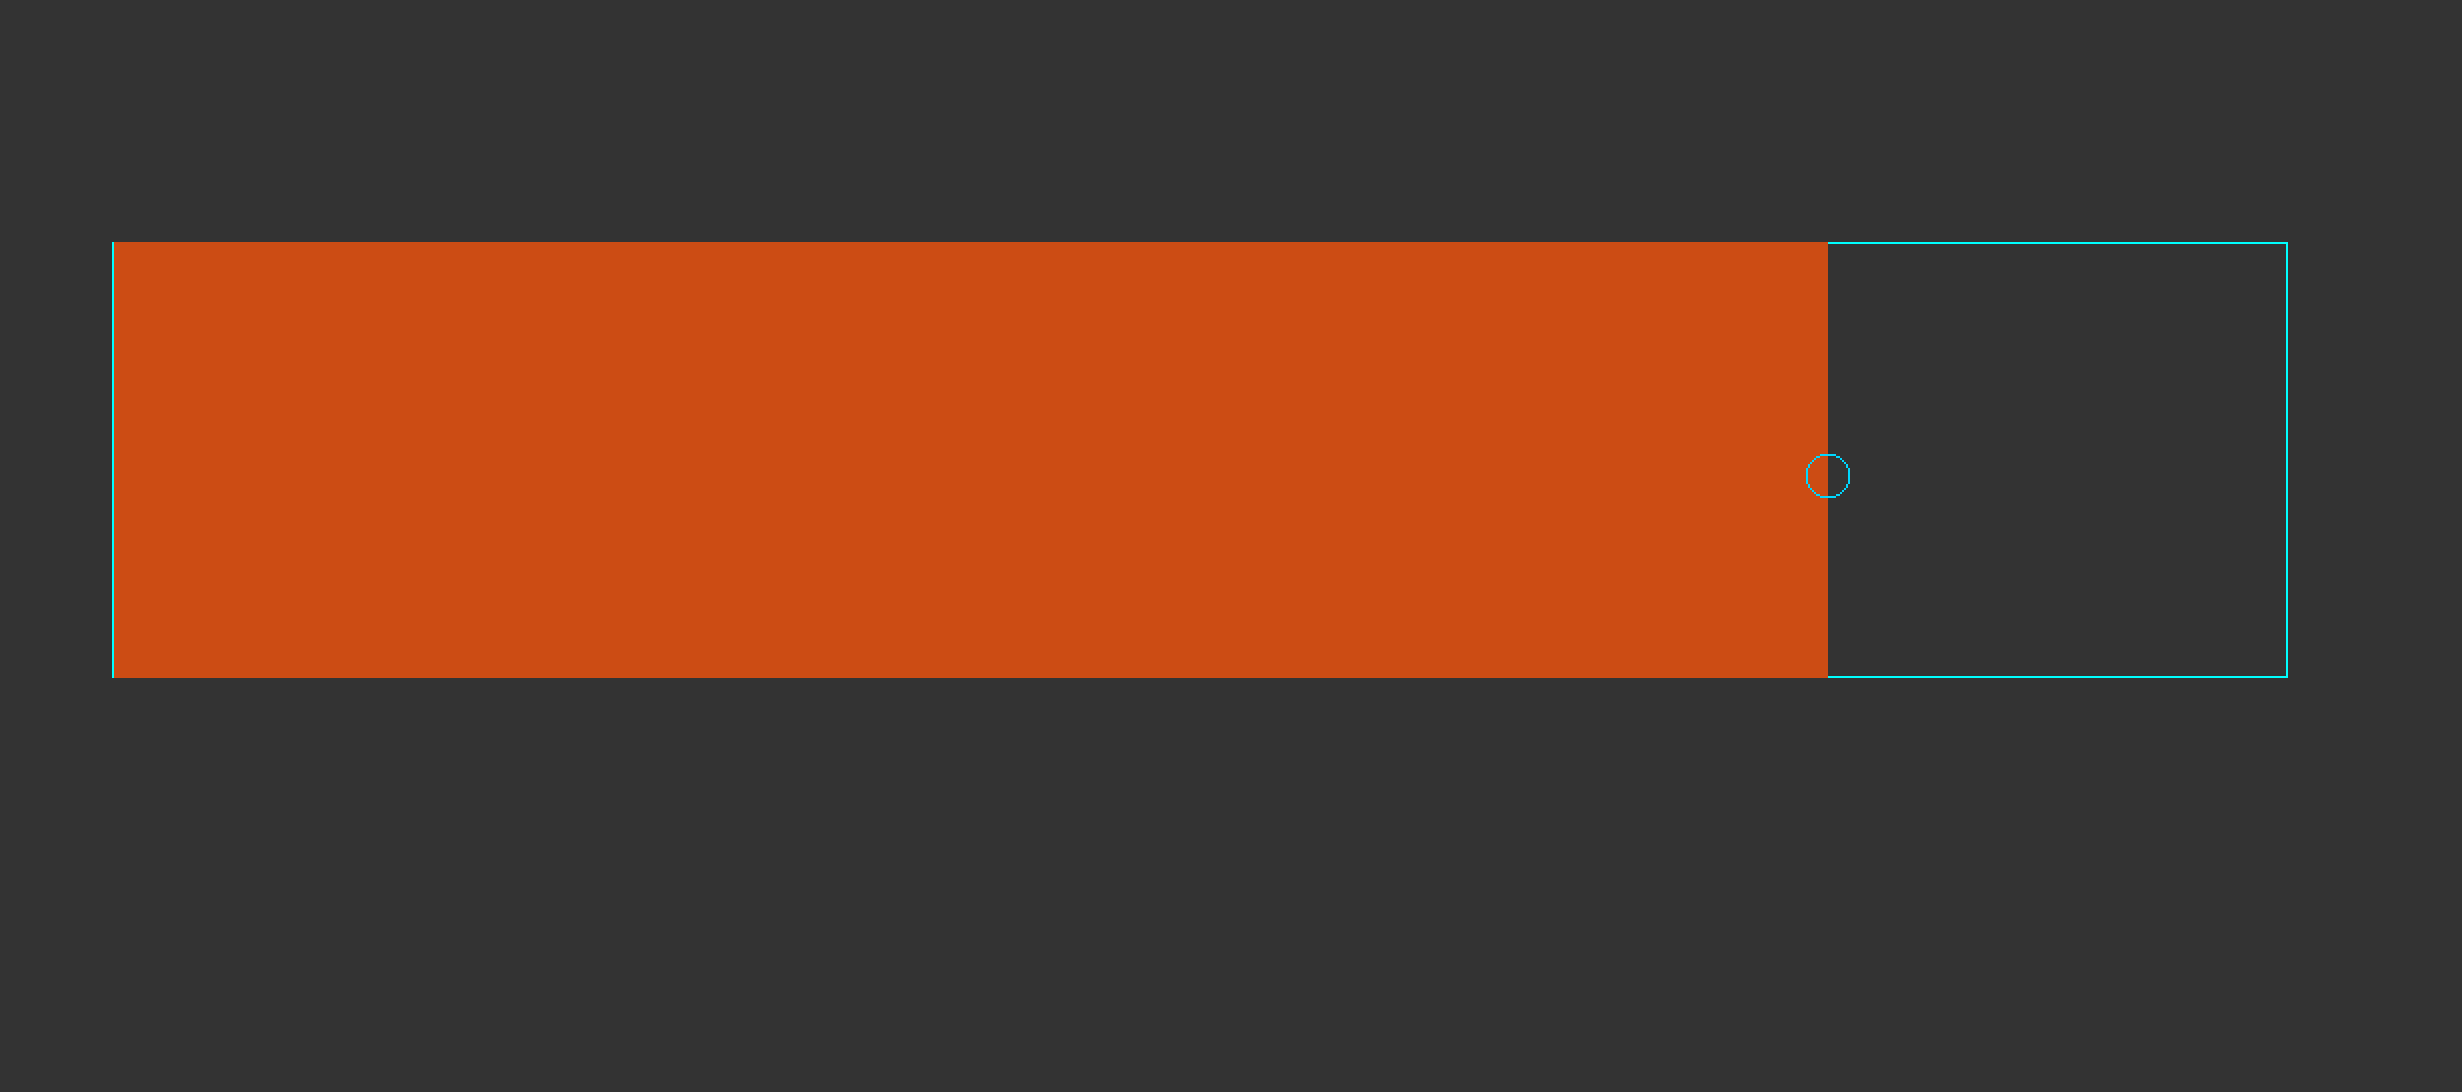
\includegraphics[width=.95\textwidth]{gfx/06_visual_representation/mpTUI_slider-onscreen.png}
			\caption{Rendu du slider dans une fenêtre OpenGL}
		\end{subfigure}%
	}
	\caption{Un simple slider dans la librairie mp.TUI}
\end{figure}


\subsection{Outils pour l'interaction multitouch}


%-------------------------- Figure : mp.TUI overview ------------------------
\begin{figure}[!htbp]
	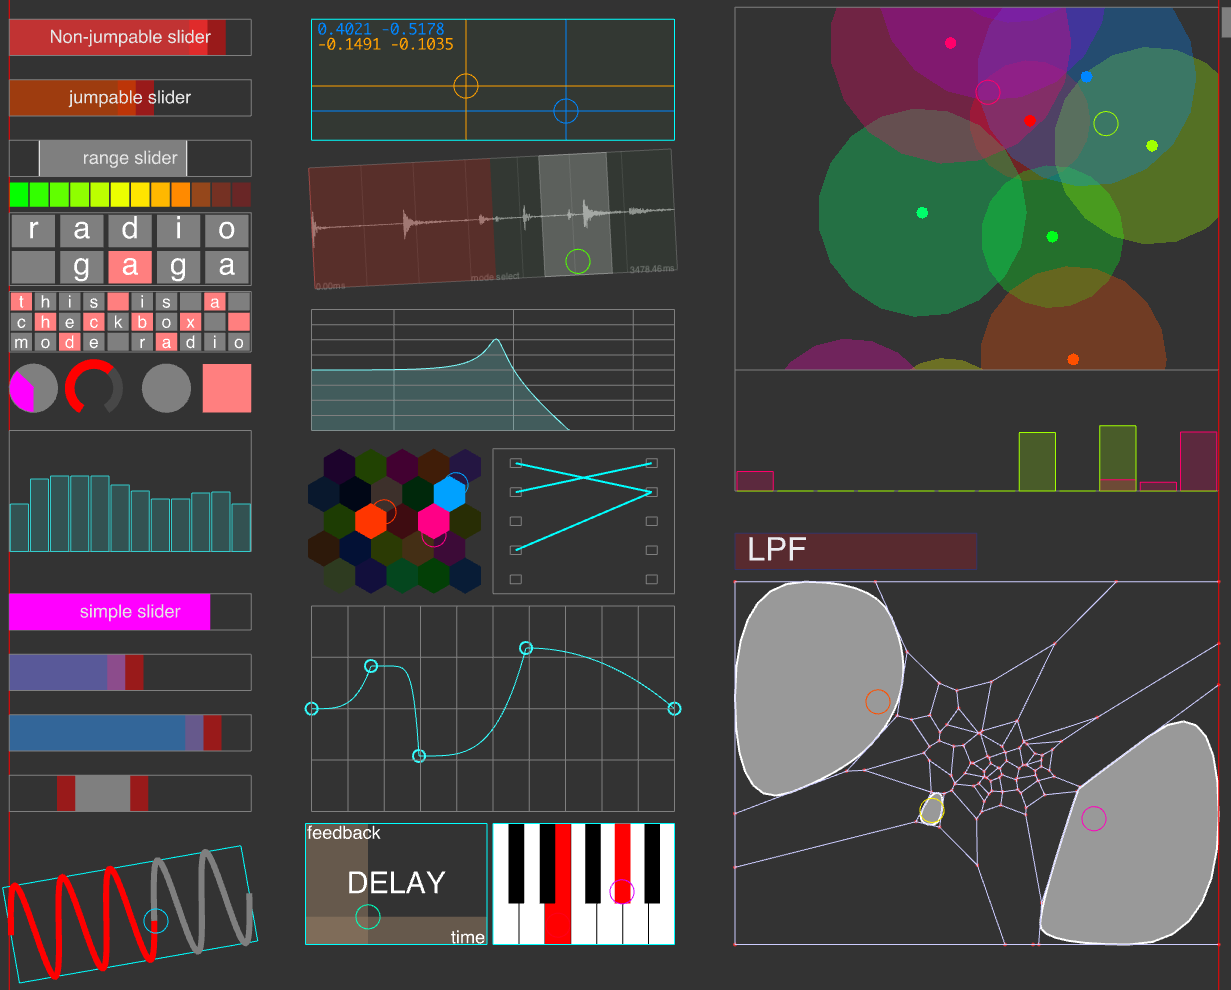
\includegraphics[width=\textwidth]{gfx/mpTUI/mp-TUI-preview.png}
	\caption{Aperçu de quelques composants graphiques de la librairie mp.TUI}
	\label{fig:visual_representation:mp.TUI}
\end{figure}

% \begin{figure}
% 	\captionsetup{format=plain}%
% 	\centering
% 	\begin{minipage}[t]{0.48\textwidth}
% 		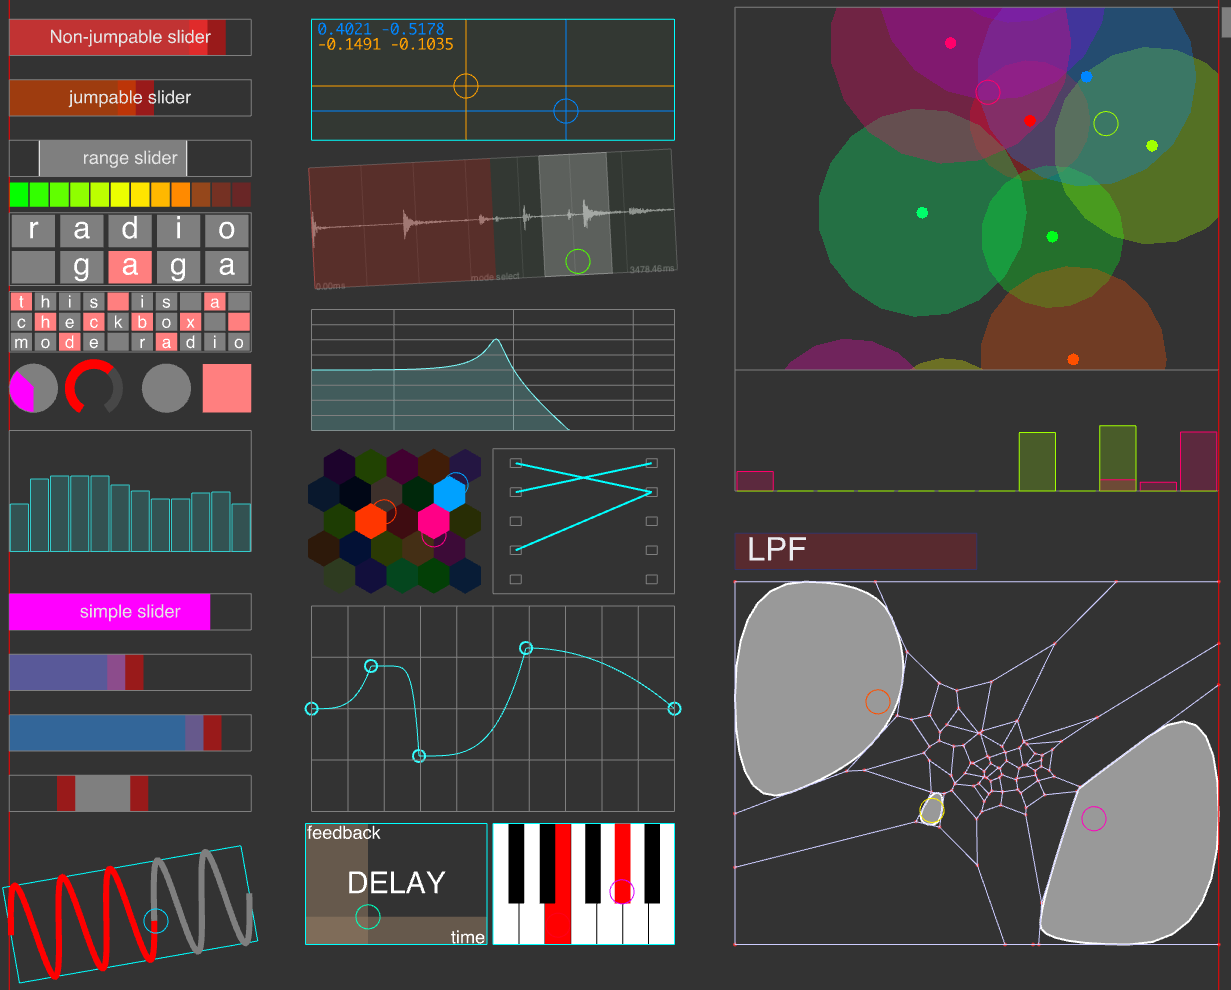
\includegraphics[width=\linewidth]{gfx/mpTUI/mp-TUI-preview.png}
% 		\captionof{figure}{Exemples de composants}	
% 		\label{fig:visual_representation:overview}
% 	\end{minipage}%
% 	\hspace{.02\linewidth}	
% 	\begin{minipage}[t]{0.48\textwidth}
% 	    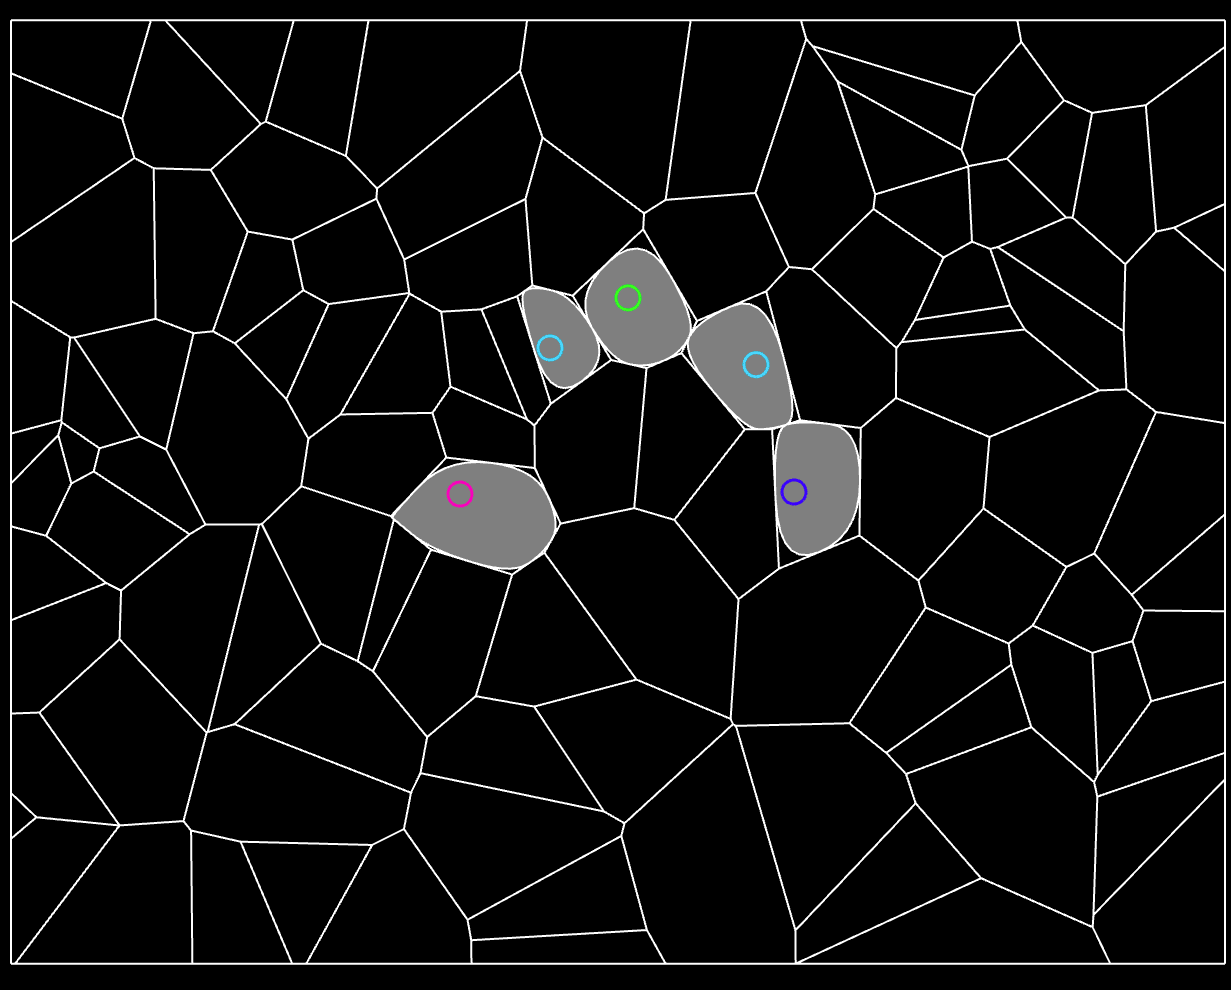
\includegraphics[width=\linewidth]{gfx/mpTUI/mp-TUI-voronoi.png}
% 		\caption{Modèle de Voronoi}
% 		\label{fig:visual_representation:voronoi}
% 	\end{minipage}
% \end{figure}

%-------------------------- Figure : groups ----------------------------------
\begin{figure}[!htbp]
	\captionsetup{format=plain}%
	\centering
	\begin{minipage}[t]{0.48\textwidth}
		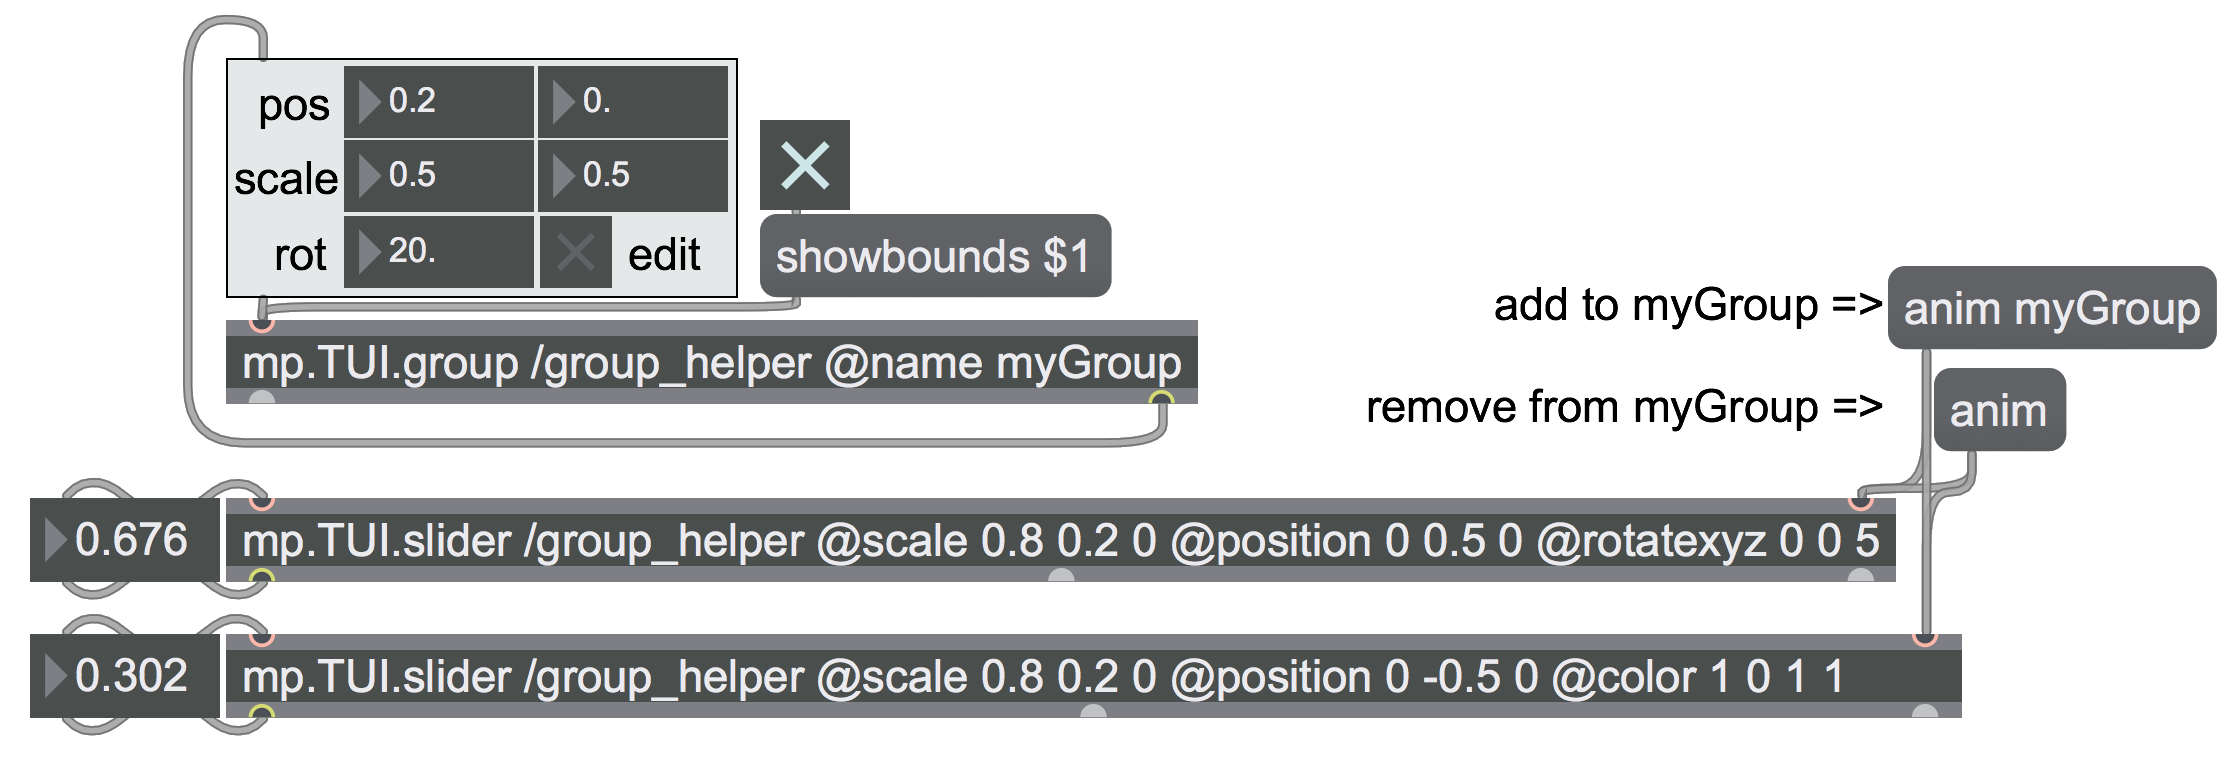
\includegraphics[width=\linewidth]{gfx/06_visual_representation/mpTUI_groups_patcher.png}
		\caption{Patch Max présentant des objets groupés}
		\label{fig:visual_representation:groups_patch}
	\end{minipage}
	\hspace{.02\linewidth}
	\begin{minipage}[t]{0.48\textwidth}
	    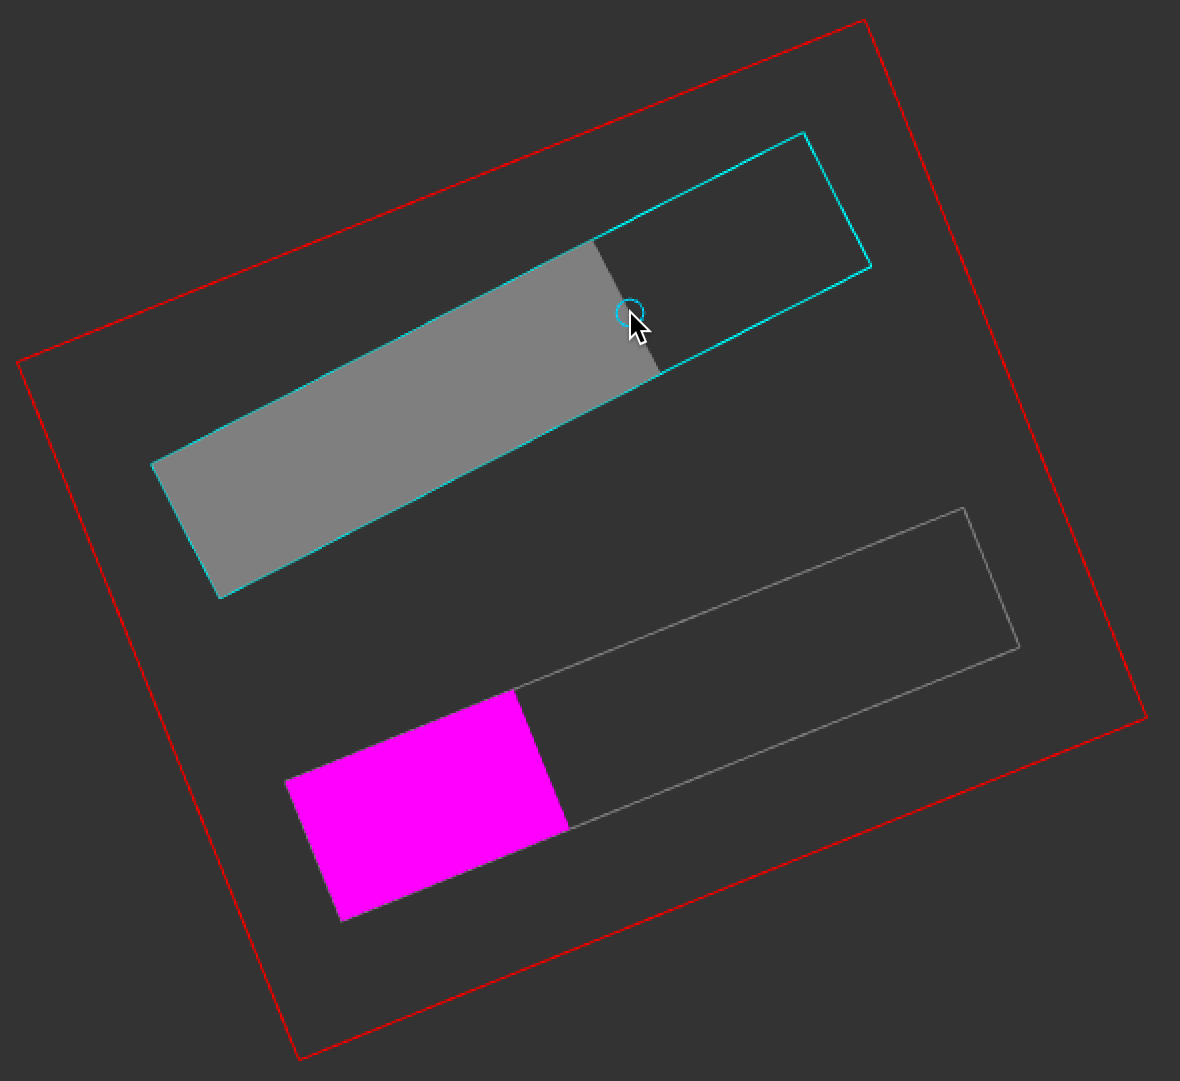
\includegraphics[width=\linewidth]{gfx/06_visual_representation/mpTUI_groups.png}
		\caption{Groupement d'objets et édition ``à la main''}
		\label{fig:visual_representation:groups}
	\end{minipage}
\end{figure}

\subsection{Instanciations dynamiques}

Utilisation de la librairie MP pour créer dynamiquement des instances éphémères de composant UI.
Exemple avec mp.TUI.canvas ou l'on vient ``piocher'' un slider créé via un objet mp.TUID.slider.
Considération pour la gestion de la destruction de ces instances.


\subsection{Performances}
La bibliothèque mp.TUI est entièrement développée avec des objets natifs de la distribution Max. Cette approche, bien que plus coûteuse en charge \gls{CPU} que des objets compilés, a l'avantage de permettre à tout utilisateur de Max de modifier facilement les composants et de les adapter à ses besoins. De plus, les composants mp.TUI s'appuient essentiellement sur OpenGL, de sorte que la majeure partie de la charge de calcul est laissée au \gls{GPU}. L'interaction tangible avec les objets de la \gls{GUI} se fait à l'aide du moteur Bullet-Physics\footnote{\url{http://bulletphysics.org/}} intégré dans Max. Bien que cela puisse être plus coûteux pour certaines formes simples, cela nous permet de concevoir des composants \gls{GUI} de n'importe quelle forme et orientation, comme des \textit{sliders} courbes ou des formes creuses, et de les animer potentiellement, comme dans l'exemple des "balles rebondissantes" où plusieurs curseurs 2D peuvent être déplacés et lancés dans une zone délimitées.

%%%%%%%%%%%%%%%%%%%%%%%%%%%%%%%%%%%%%%%%%
\section*{miscellanées (temporaire à supprimer)}
citations :

The  keyboards  were  always  there...  for  some  reason  or  other  it  looks  good  if  you’re playing a keyboard. People understand then you’re making music.” Robert Moog in Trevor Pinch, “Why You Go to a Piano Store to Buy a Synthesizer: Path Dependence and the Social Construction of Technology,” in Path Dependence and Creation


NIME 2019 : ``From Mondrian to Modular Synth: Rendering NIME using Generative Adversarial Networks''

Chamagne

\begin{quote}
Visual language is one of the oldest forms of knowledge representation and predates conventional written language by almost 25,000 years
\end{quote}
\cite{tufte_visual_2001}

\cite{moody_physics_2009}


\begin{quotation}
If you ask the man on the stree "What's a synthesizer?" He will reply "A synthesizer is a keyboard instrument"... If you go in a retail store ad say I want to see some electronic instruments, they'll send you to the keyboard department, because a synthesizer is a keyboard instrument by default. — Don Buchla, synthesizer pioneer (interview)
\end{quotation}
\cite{pinch_why_2001}